\subsection{Universal CVSS Calculator} \label{subsec:projektbericht-loesungsweg-typescript-cvss-online-calculator}

Dieses Kapitel geht auf die Details hinter der CVSS-Implementierung in TypeScript\footnote{\url{https://github.com/org-metaeffekt/metaeffekt-universal-cvss-calculator}} ein, wie sie im Universal CVSS Calculator\footnote{\url{https://www.metaeffekt.com/security/cvss/calculator}} der {\metaeffekt} verwendet wird.
In Abbildung \ref{fig:cvss-ts-calculator-class-diagram} kann das Klassendiagramm der TypeScript-Klassen mit allen Exports und Imports gefunden werden, über welche es in diesem Kapitel gehen wird.

Da sich die Vektoren nur in ihren verwendeten Metriken, Metrikgruppen und der Score-Berechnung unterscheiden, kann recht viel der gemeinsamen Logik in eine Oberklasse \code{CvssVector} extrahiert werden.


\begin{figure}[htbp] % here, top, bottom, separate page
    \centering
    \makebox[\textwidth][c]{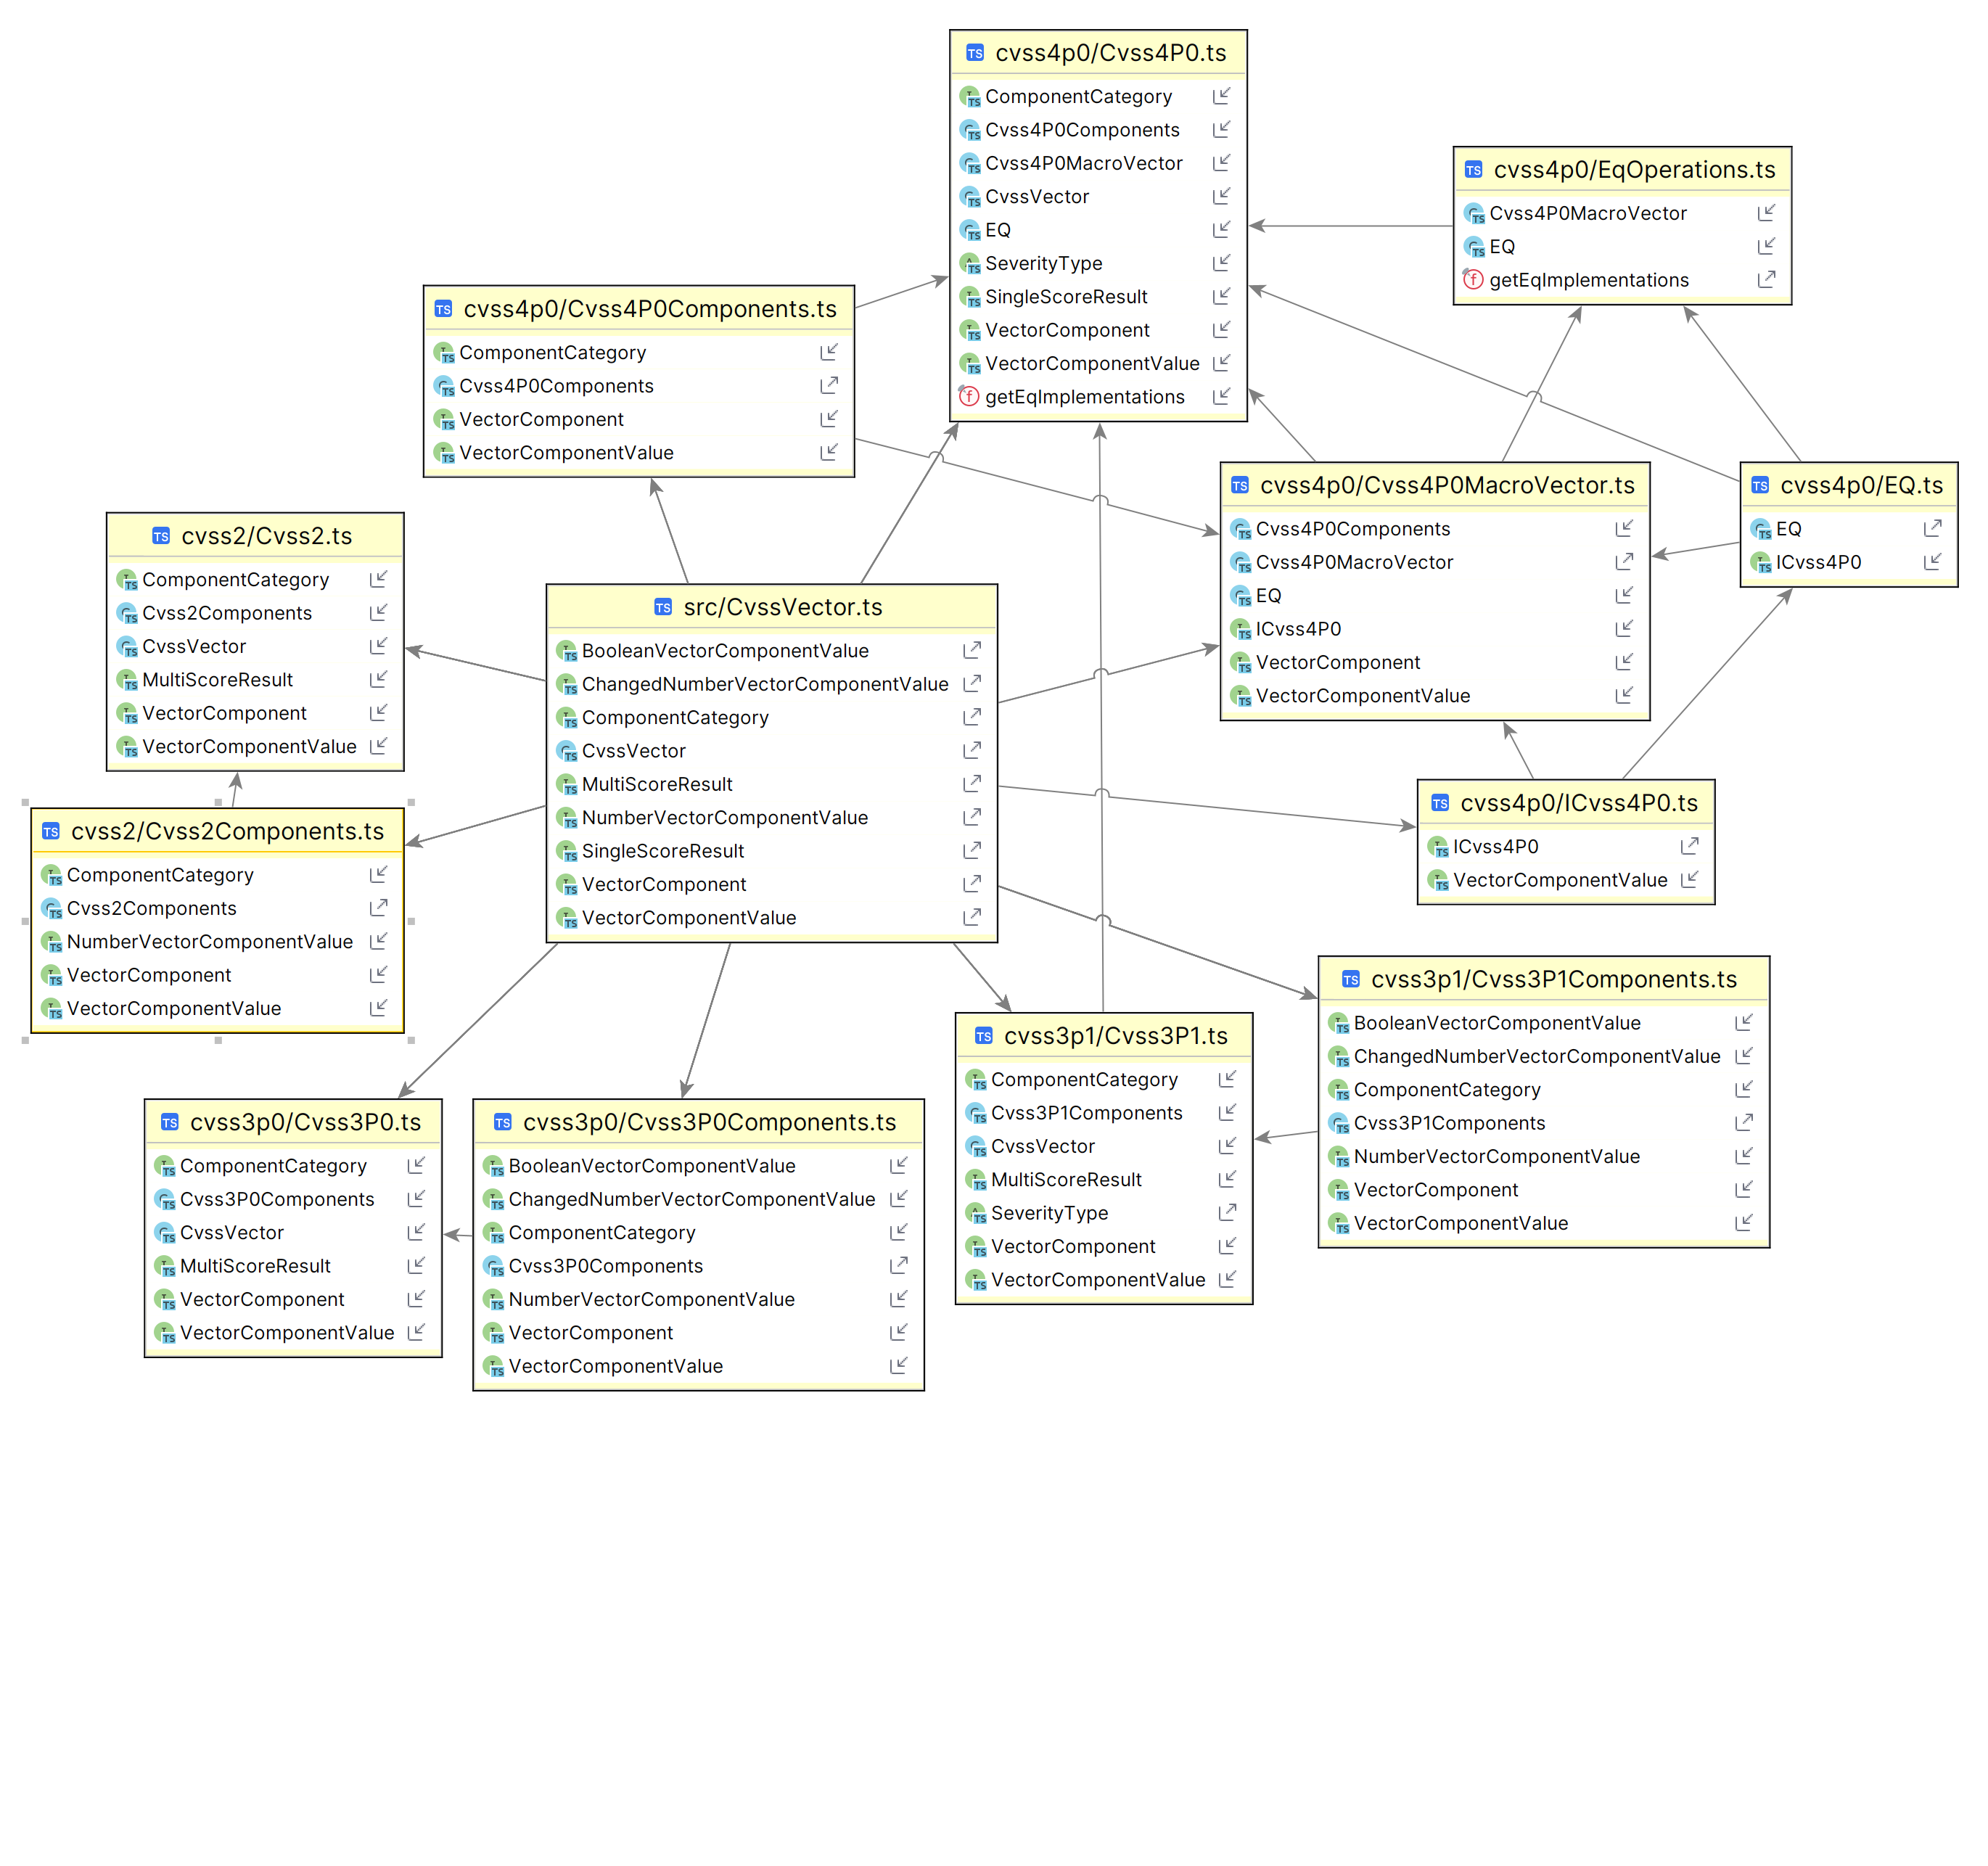
\includegraphics[width=1.2\textwidth, keepaspectratio]{res/grafiken/cvss-ts-calculator-class-diagram}}
    \caption{Klassendiagramm des CVSS-Rechners in TypeScript}
    \label{fig:cvss-ts-calculator-class-diagram}
\end{figure}

